\section{Методика использования программного средства}
\label{sec:manual}

В данном разделе приведены основные сведения по работе с программным средством.

Для того чтобы воспользоваться приложением данного дипломного проекта, требуется установить приложение Telegram для любой из следующих платформ:

\begin{itemize}
	\item iOS;
	\item Android;
	\item Windows;
	\item Linux;
	\item Web-клиент.
\end{itemize}

Далее рассмотрены основные функции, предоставляемые приложением пользователям.

При старте чата с ботом отображается сообщение с основными функциями бота (рисунок \ref{fig:manual:agenda_screen}).

\begin{figure}[ht]
\centering
	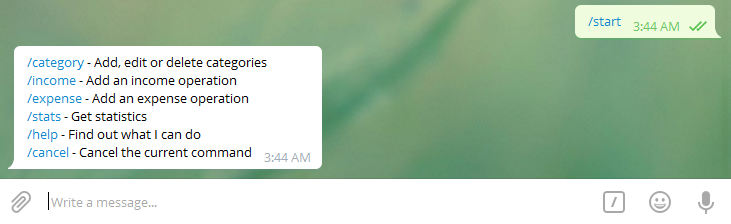
\includegraphics[scale=0.7]{agenda_screen.png}
	\caption{Сообщение с основными функциями бота}
	\label{fig:manual:agenda_screen}
\end{figure}

Для удобства использования в строке ввода сообщения присутствует кнопка просмотра доступных команд. Для того, чтобы воспользоваться командой, достаточно нажать на одну из предложенных кнопок (рисунок \ref{fig:manual:command_buttons}).

\begin{figure}[ht]
\centering
	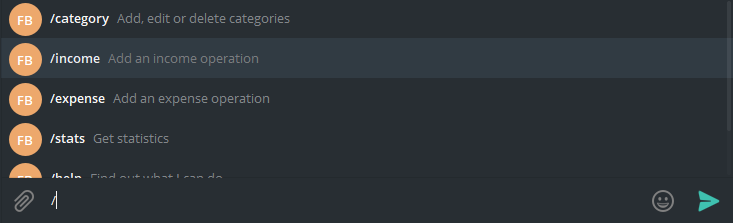
\includegraphics[scale=0.7]{command_buttons.png}
	\caption{Вспомогательное меню с доступными командами}
	\label{fig:manual:command_buttons}
\end{figure}

Любую из команд можно отменить, введя команду /cancel, либо выбрав её из вспомогательного меню, как показано на рисунке \ref{fig:manual:cancel_button}. 

\begin{figure}[ht]
\centering
	
\includegraphics[scale=0.7]{cancel_button.png}
	\caption{Вызов функции отмены}
	\label{fig:manual:cancel_button}
\end{figure}

Добавление категорий происходит путём выбора команды /category и последовательных ответов на вопросы в диалоге настройки. Ответы можно давать нажимая на кнопки, предлагаемые ботом, либо вводить через поле ввода. Процесс создания категории показан на рисунке \ref{fig:manual:category_creating}.

\begin{figure}[ht]
\centering
	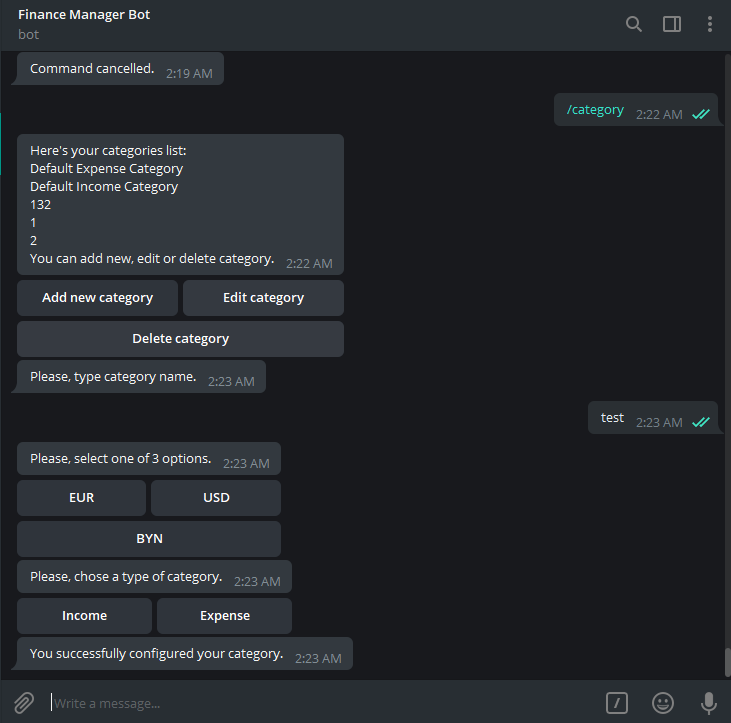
\includegraphics[scale=0.7]{category_creating.png}
	\caption{Процесс создания категории}
	\label{fig:manual:category_creating}
\end{figure}

Добавление операций в категории происходит путём выбора команды /income для категорий-доходов либо /expense для категорий-расходов. Процесс добавления операции в категорию показан на рисунке \ref{fig:manual:operation_creating}.

\begin{figure}[ht]
\centering
	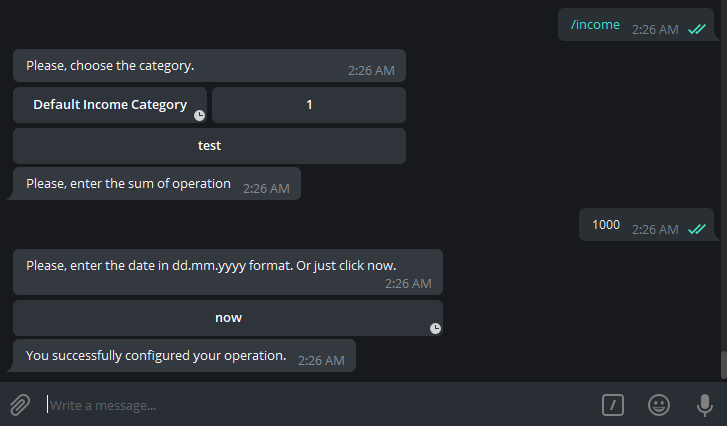
\includegraphics[scale=0.7]{operation_creating.png}
	\caption{Процесс создания операции}
	\label{fig:manual:operation_creating}
\end{figure}

Для просмотра статистики, необходимо воспользоваться командой /stats. В зависимости от цели, требуется выбрать один из пунктов контекстного меню. Если подробная статистика по операциям пользователя не интересует, он может воспользоваться функцией показа статистики по типам категорий. 

В случае, если пользователя интересует подробная статистика, ему следует выбрать категорию, для которой статистика будет выведена. После выбора категории, пользователю будет показан список операций с суммами и датами добавления. Для категорий-доходов сумма будет отображаться со знаком плюс, для категорий-расходов сумма будет отображаться со знаком минус.

Таким образом, в данном разделе приведены примеры использования некоторых их основных возможностей разработанного программного средства. Следование им должно значительно упростить выполнение некоторых рутинных задач слежения за персональными расходами.
